\documentclass[tikz,border=8pt]{standalone}
\usepackage{tikz}
\usepackage{amsmath}
\usepackage{xcolor}
\usetikzlibrary{positioning}
\begin{document}
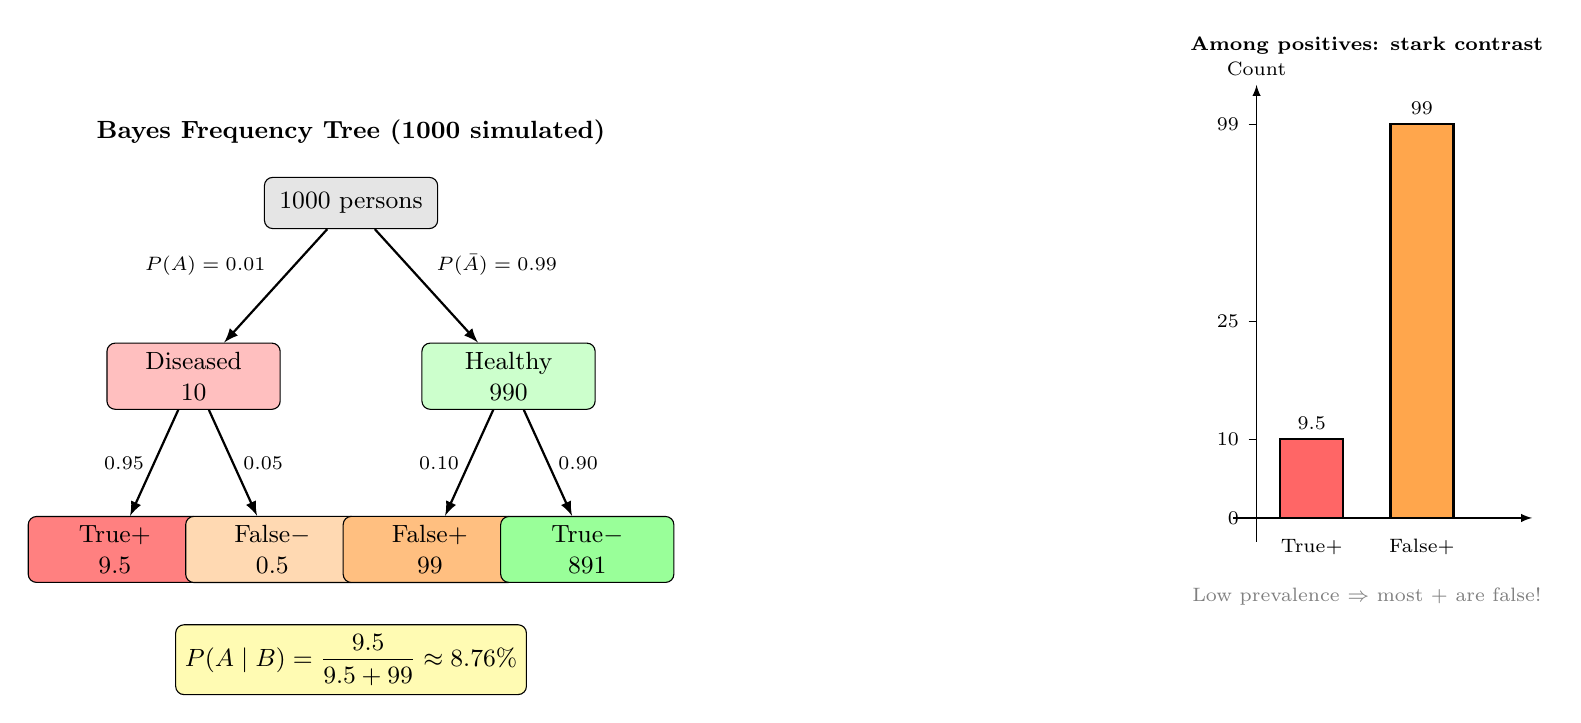
\begin{tikzpicture}[
  box/.style={draw,rounded corners=3pt,minimum width=2.2cm,minimum height=0.65cm,
              font=\small,align=center},
  lbl/.style={font=\scriptsize,align=center},
  >=latex
]

  %% ===== LEFT PANEL: Frequency Tree =====

  % Root: 1000 people
  \node[box,fill=gray!20] (root) at (-5,0) {1000 persons};

  % Level 1: diseased / healthy
  \node[box,fill=red!25] (dis) at (-7,-2.2) {Diseased\\10};
  \node[box,fill=green!20] (hlth) at (-3,-2.2) {Healthy\\990};

  \draw[->,thick] (root) -- node[lbl,above left] {$P(A)=0.01$} (dis);
  \draw[->,thick] (root) -- node[lbl,above right] {$P(\bar{A})=0.99$} (hlth);

  % Level 2 from diseased
  \node[box,fill=red!50] (tp) at (-8,-4.4) {True$+$\\9.5};
  \node[box,fill=orange!30] (fn) at (-6,-4.4) {False$-$\\0.5};

  \draw[->,thick] (dis) -- node[lbl,left,pos=0.5] {$0.95$} (tp);
  \draw[->,thick] (dis) -- node[lbl,right,pos=0.5] {$0.05$} (fn);

  % Level 2 from healthy
  \node[box,fill=orange!50] (fp) at (-4,-4.4) {False$+$\\99};
  \node[box,fill=green!40] (tn) at (-2,-4.4) {True$-$\\891};

  \draw[->,thick] (hlth) -- node[lbl,left,pos=0.5] {$0.10$} (fp);
  \draw[->,thick] (hlth) -- node[lbl,right,pos=0.5] {$0.90$} (tn);

  % Panel title
  \node[font=\bfseries\small] at (-5,0.9) {Bayes Frequency Tree (1000 simulated)};

  % Bayes result annotation
  \node[font=\small,align=center,fill=yellow!30,draw,rounded corners=3pt]
    at (-5,-5.8)
    {$P(A\mid B) = \dfrac{9.5}{9.5+99} \approx 8.76\%$};

  %% ===== RIGHT PANEL: Contrast bar chart =====
  \begin{scope}[shift={(6.5,-4.0)}]

    % axes
    \draw[->] (-0.3,0) -- (3.5,0) node[right,font=\scriptsize] {};
    \draw[->] (0,-0.3) -- (0,5.5) node[above,font=\scriptsize] {Count};

    % True positive bar (9.5)
    \fill[red!60] (0.3,0) rectangle (1.1,1.0);
    \draw[thick] (0.3,0) rectangle (1.1,1.0);
    \node[font=\scriptsize,above] at (0.7,1.0) {9.5};
    \node[font=\scriptsize,below,align=center] at (0.7,-0.15) {True$+$};

    % False positive bar (99)
    \fill[orange!70] (1.7,0) rectangle (2.5,5.0);
    \draw[thick] (1.7,0) rectangle (2.5,5.0);
    \node[font=\scriptsize,above] at (2.1,5.0) {99};
    \node[font=\scriptsize,below,align=center] at (2.1,-0.15) {False$+$};

    % y ticks
    \foreach \y/\lbl in {0/0,1.0/10,2.5/25,5.0/99} {
      \draw (-0.1,\y) -- (0,\y);
      \node[font=\scriptsize,left] at (-0.1,\y) {\lbl};
    }

    \node[font=\bfseries\scriptsize,align=center] at (1.4,6.0)
      {Among positives: stark contrast};
    \node[font=\scriptsize,align=center,gray] at (1.4,-1.0)
      {Low prevalence $\Rightarrow$ most $+$ are false!};

  \end{scope}

\end{tikzpicture}
\end{document}
